\documentclass[aspectratio=169,11pt]{beamer}

\usetheme{metropolis}
\usepackage[utf8]{inputenc}
\usepackage[T1]{fontenc}
\usepackage[french]{babel}
\usepackage{graphicx}

% Couleur principale (bleu hospitalier)
\definecolor{picu}{HTML}{1A73E8}
\setbeamercolor{frametitle}{bg=picu}
\setbeamercolor{progress bar}{fg=picu}

\title{PICU}
\subtitle{Plateforme Intelligente de Coordination des Urgences}
\author{Younes Basir}
\institute{Université Privée de Fès \textperiodcentered{} CHU Hassan II de Fès}
\date{Année universitaire 2024-2025}

\begin{document}

\maketitle

\begin{frame}{Problématique}
  Comment coordonner les urgences en temps réel, assister le triage par
  l'IA, et garantir un workflow fiable et traçable ?

  \vspace{0.5cm}
  \begin{itemize}
    \item centraliser patients, visites, ressources et personnel
    \item workflow transactionnel explicite et auditable
    \item assistance IA \textbf{supervisée}
  \end{itemize}
\end{frame}

\begin{frame}{Workflow de la visite}
  \begin{center}
    \texttt{waiting} $\rightarrow$ \texttt{placed} $\rightarrow$
    \texttt{in\_treatment} $\rightarrow$ \texttt{discharged}

    \vspace{0.5cm}
    % Image optionnelle (deja presente dans rapport-stage/images/)
    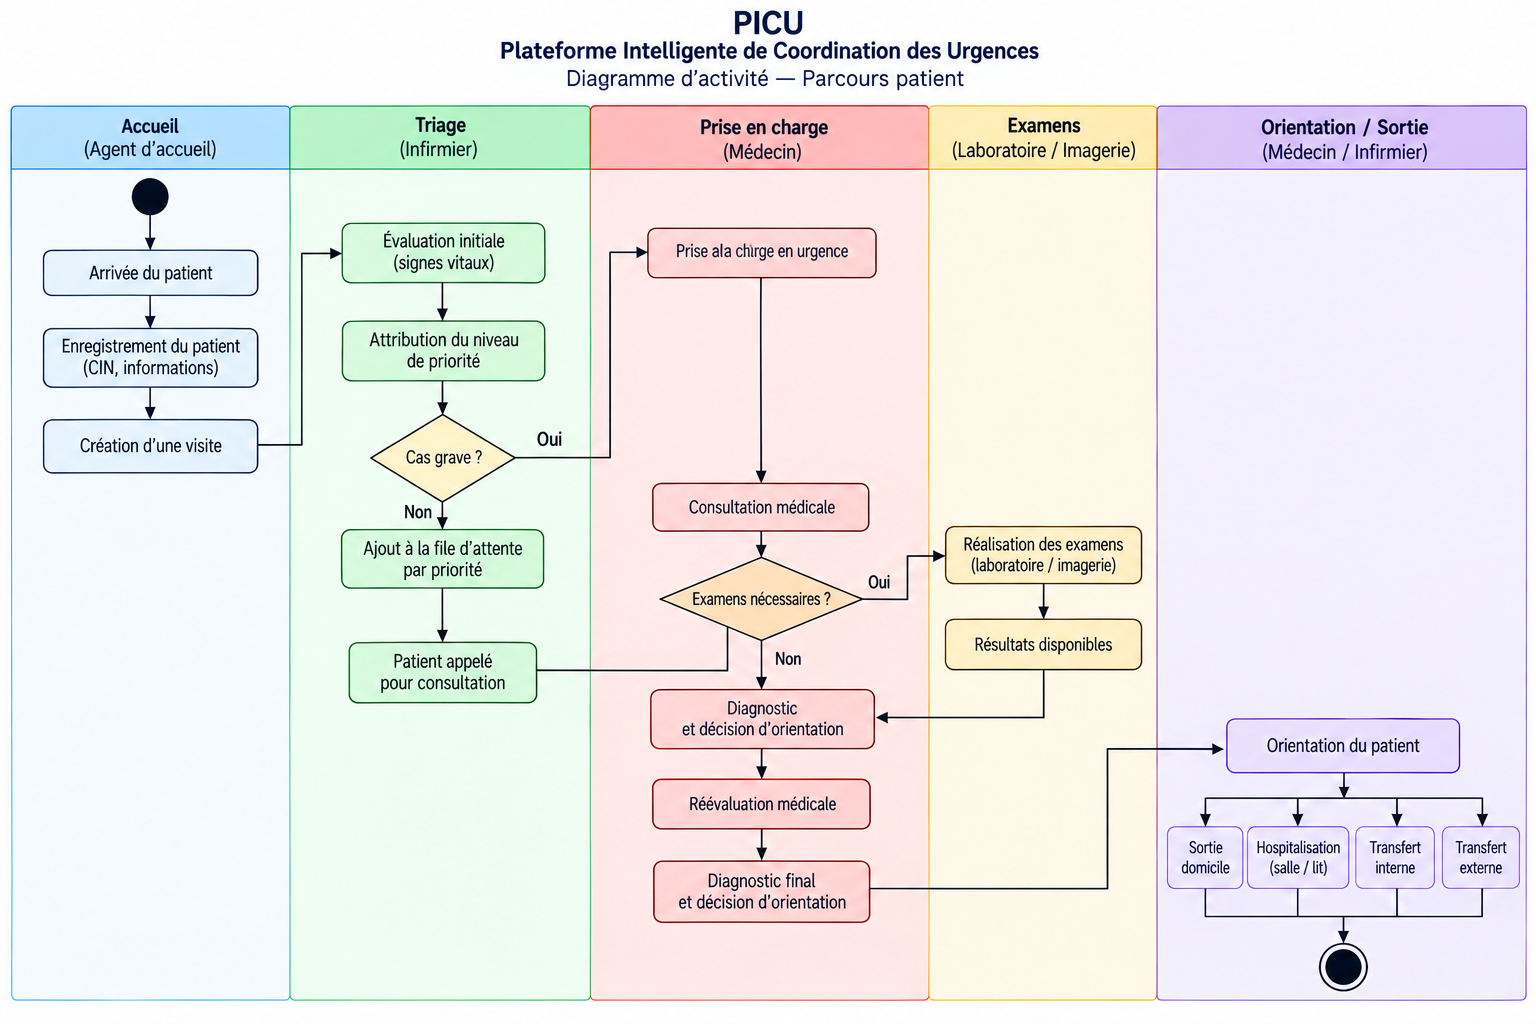
\includegraphics[width=0.55\textwidth]{../images/activity_diagram.png}
  \end{center}
\end{frame}

\end{document}
